\documentclass[11pt,twoside]{report}
\usepackage{preamble}
\graphicspath{{../img/ch3/}}
\setcounter{chapter}{2}


\begin{document}

\chapter{Fish behaviours in 2D}

The vast majority of the collective behaviour of fish were performed in a quasi--2D environment, where the fish were confined in a shallow water tank. The motions of the fish can be captured by digital cameras and analysed by tracking softwares.

\section{Methods for 2D Data}

\subsection{Basic Image Processing}

To get useful information out of the image, we want to transform the video, where the fish appear as a dark spot, into a better representation. Ideally, the processed image should be a collection of delta functions, where the pixel intensity in the centres of each individual fish is maximum, and the pixel intensities are zero everywhere else. Even though it is possible to construct such transformation directly with machine learning based approaches \cite{newby2018}, it is still not a straightforward and easy task. Traditional image processing methods such as thresholding, blurring, and morphological operations were still applied a lot in this project. As a result, I get a video where each fish have high pixel intensity values and the background intensity values are zero. Figure \ref{fig:2d_process} illustrate the result of the transformation. On the left side is the video recorded during the experiment, and the central image is the ``foreground'' after the image processing, where the background is removed.

I obtained the foreground videos of the fish with two different steps, the removal of the background and removal of the noises. The background is defined as the temporal average of the image, since the fish are constantly moving while rest of the scene is static. In order to tackle the varying illumination conditions\marginfootnote{
The brightness level fluctuates even I keep the illumination setting unchanged in the laboratory. In a relatively dark ($\sim$20 lux) condition, those fluctuations could not be ignored.
}, I take a running average of a time--window, instead of calculating the overall average. The pixel intensity of the background at time $t$, of pixel $(x, y)$, can be written as

\begin{equation}
I_\mathrm{bg}(t; x, y) = \frac{1}{T} \sum_{\tau=t}^{t+T}{I(\tau; x, y)}
\end{equation}

\noindent where $I(\tau; x, y)$ is the pixel intensity of the video at time $\tau$ in position $(x, y)$, and $T$ is the duration of the window, usually taken as 40 seconds. The difference between the background video and original video yields a foreground video, written as

\begin{equation}
	I_\mathrm{fg}(t; x, y) = I_\mathrm{bg}(t; x, y) - I(t; x, y)
\end{equation}

\noindent and the order of the subtraction ensures the fish, originally appear darker in the video, would be represented by brighter pixels in the foreground video, shown in the centra image in Fig.\ \ref{fig:2d_process}. The subtraction result are often very noisy. To remove the noise, I applied gaussian filter to the foreground image, to smooth the sharp noises. Additionally, I applied the a combination of OTSU threshold and local gaussian threshold to separate the pixels belonging to the fish and other pixels. The OTSU threshold separate all the pixels into different groups to minimise the inter--group variance of the intensity distribution. LOCAL THRESHOLD.

\begin{SCfigure}
  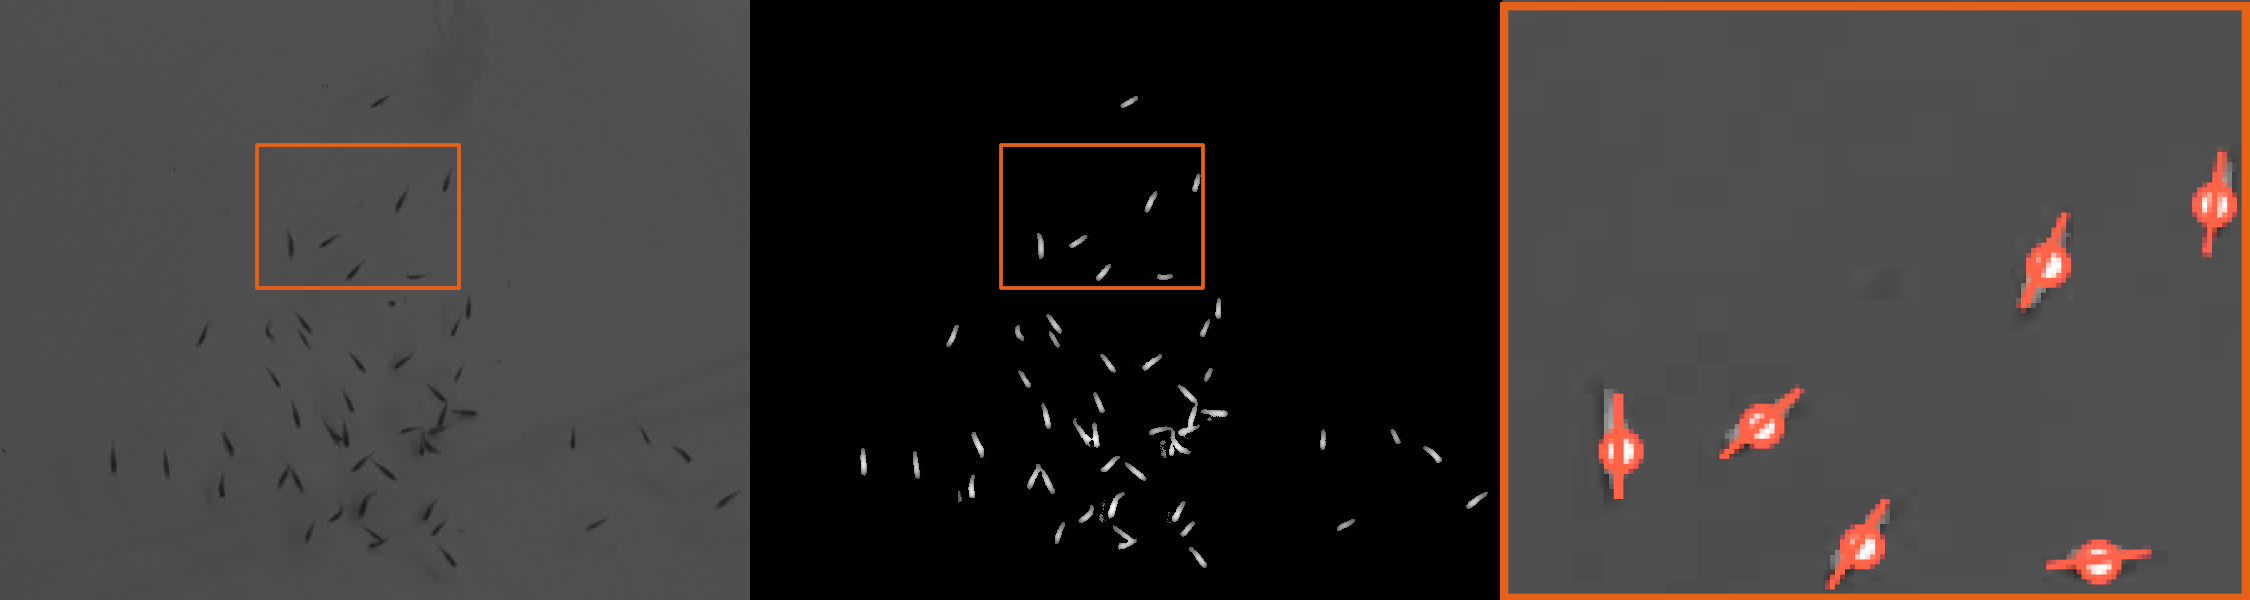
\includegraphics[width=\linewidth,outer]{2d-processing.png}
  \caption{}
  \label{fig:2d_process}
\end{SCfigure}


\subsection{Extracting Features}

From the processed video, it is to possible extract the features\marginfootnote{
In the computer vision community, people call the locations of objects ``features''. This slightly odd name roots in the 3D reconstruction problem, which will be discussed in the next chapter. Very briefly, we can not recover 3D geometry from the background, like a purely white wall, where all the pixels have the same intensity value. Instead, some ``features'', with intensity gradients, are required\cite{ma2005}. Adapting this naming tradition, the positions of the fish in 2D images will be called ``features''. An alternative name would be the just the ``positions''. However, the selected name stressed the nature of a fish image in the photo: it is a ``feature'' of the photo, but not a (3 dimensional) position of a fish.
} in each frame that corresponds to the fish. In order to tackle the problem, we employed a method that not only capture the positions, but also the information of the fish orientations and body shapes.

the shape invariant features offered great way to locate fish in a ``dense'' system.

\section{Methods for both 2D and 3D data}

This section will introduce the algorithms that are used for both 2D experiments and the 3D analysis of fish behaviours, which would be discussed in the next chapter.

\subsection{Linking Positions to Trajectories}

\subsection{Removing Overlapped Particles}

I used linear programming method to remove overlapped Particles. Supposing there are $N$ particles in total, and we wish to find $K$ non--overlapping particles, where each particle has an uncertainty value of $e_i$. The task can be written as a linear programming problem with quadratic constrains as follows:

\begin{equation}
\begin{aligned}
	\textrm{Minimize} && \sum_i{e_i x_i} \\
	\textrm{Subject to} && d_{12} x_1 x_2 \le \sigma \\
	&& d_{13} x_1 x_3 \le \sigma \\
	&& \vdots  \\
	&& d_{ij} x_i x_j \le \sigma \\
	&& \sum_i{x_i} = K
\end{aligned}
\end{equation}

An alternative choice is to apply a greedy algorithm\marginfootnote{
An anonymous physicist implemented this greedy algorithm, and named it \texttt{musicalChair} confusingly, in a custom particle tracking code.
}: always remove the worst match until there is no overlap. Comparing with the greedy algorithm, the linear programming method might find a more global minimum.

\subsection{Possible Improvements}

\subsubsection{Neural Network}

There are two steps in the image processing that can be improved in the image processing pipeline. The first one is the removal of background. In my current method, I calculated a rolling average of the entire video. The window size of the averaging operation is set by the user, which is very difficult to optimise because the video processing typically takes hours to finish. Practically, a rule-of-thumb number (600 frames) was applied. However, the fish in the video are very distinct from their background, and it is an easy task for people to spot the fish in a static image. This suggests a static image contains enough information to distinguish the foreground (fish) and background (tank). 

The neural network is very suitable for extracting the needed information in our case. Developed in the 1980s and revived very recently (2010).

\subsubsection{Hierarchical Shape Matching}

In the current method, the shape templates were generated from clustering the features in a low--dimensional space.


\printbibliography

\end{document}